\chapter{Softwarewijzigingsproces}
Van software in 2018 wordt verwacht dat deze constant geupdate blijft met onder andere nieuwe features en security patches.
Om te zorgen dat dit proces goed verloopt geeft dit hoofdstuk weer hoe een verandering aan de software gemaakt kan worden.

\section{Een eigen branch in Git}
De applicatie staat in het versiebeheer systeem Git, met Git is er de mogelijkheid om geisoleerd van andere veranderingen een wijziging te maken, dit heet dan een branch. 
Zoals uitgelegd in \cref{hfd:vcs} komt elke nieuwe wijziging normaal gesproken in een nieuwe branch (tenzij dit een hotfix is).
Je kan naar een nieuwe branch wisselen met het commando \textit{git checkout -b DEV-(naam)}.
Op deze manier komt de structuur eruit te zien zoals in \cref{fig:BranchScheme}.
In deze branch kun je vervolgens ongestoord je verandering maken.

\section{Mergen via een pullrequest}
Nadat je klaar bent met ontwikkelen van je feature kun je de unittests uitvoeren.
Als deze slagen kan je een pull request maken, met een pull request kunnen anderen jouw verandering bekijken voordat zij deze daadwerkelijk toevoegen aan de codebase.
Een pull request geeft ook de mogelijkheid te discussieren.
Een pull request moet eerst acceptatie krijgen van een ander lid binnen het ontwikkelteam om deze toe te voegen aan de development branch.
\begin{figure}[h]
	\centering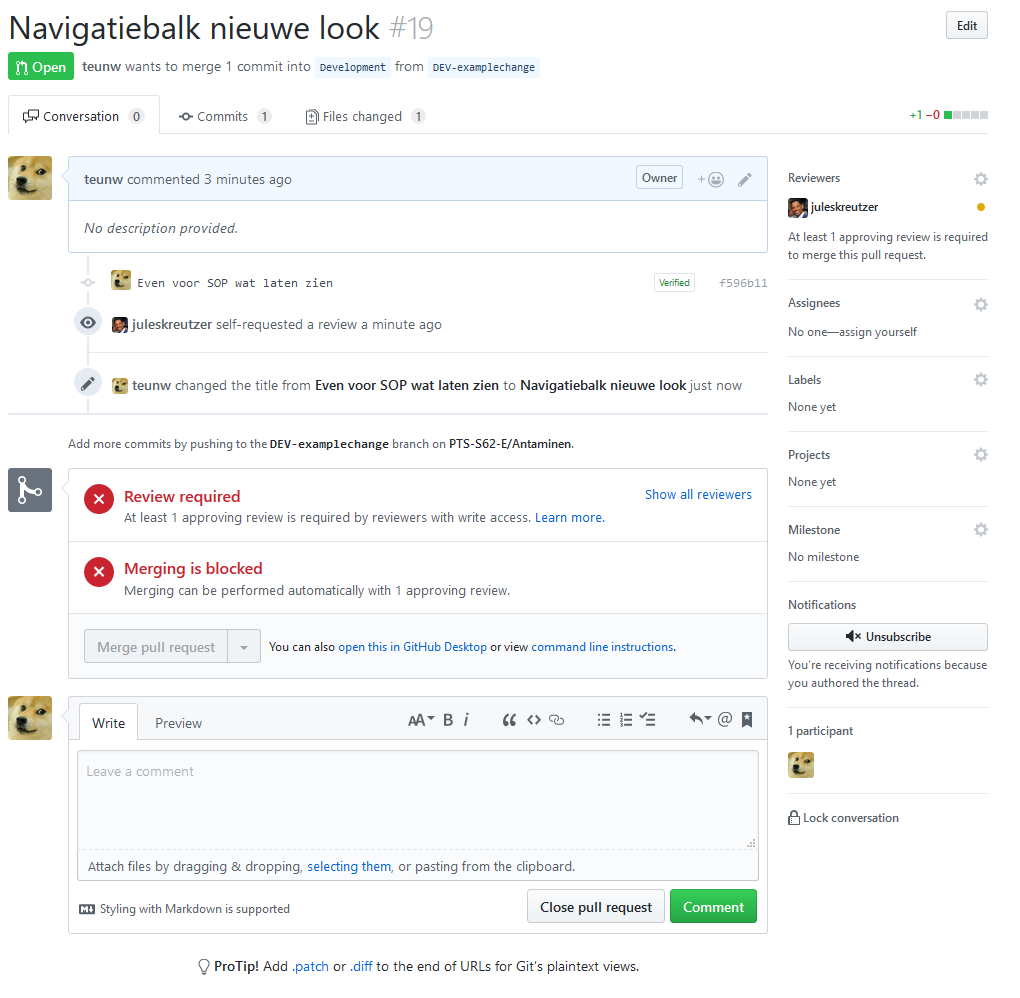
\includegraphics[width=0.6\textwidth]{images/PullRequestExample.png}
	\caption{Een voorbeeld pull request}
\end{figure}

\clearpage
\section{Acceptatietesting via staging branch}
Nadat de veranderingen uit de development branch zijn ge-unittest en afgerond zijn kan de development branch gemerged worden naar staging.
Binnen de staging omgeving wordt er gekeken of:
\begin{itemize}
	\item Er voldaan is aan de user stories.
	\item De product owner tevreden is met het resultaat.
	\item Of de veranderingen kunnen worden gedeployed op de productieomgeving.
\end{itemize}

\section{In productie}
Zodra alle stakeholders tevreden zijn met de applicatie in de staging branch kan deze worden gepushed naar productie.
Binnen de productie branch kan niet direct gepushed worden, maar merge requests kunnen er wel naartoe gemaakt worden als hotfixes. Hotfixes worden toegepast wanneer er een kritieke fout in de applicatie is ontdekt, zodat deze fout zo snel mogelijk gerepareert is.